%\documentclass{article}
%%\usepackage[html,png]{tex4ht}
%\usepackage{hyperref}
%\setlength\parindent{0pt}
%
%\title{Capped Nanotubes}
%\date{}
%\begin{document}
%\maketitle

\subsection{Capped Nanotubes}\label{cappednanotubes}

%The capped nanotube structure is the only structure that has associated child structures; a \textit{nanotube} and two \textit{cap} structures (labelled \textit{primary} and \textit{secondary}). The nanotube structure is the same class as that constructed during the isolated nanotube construction, apart from the nanotube always being of finite length. The cap structures can only be constructed as part of the parent capped nanotube structure.  
%
%As with the construction of fullerenes, capped nanotubes are either produced individually or by generating a series of structures for a given chirality and number of cap atoms.
%
%A single capped nanotube is constructed via:
%
%\textbf{File--$>$New Structure--$>$Single Structure}
%
%then click \textit{Capped Nanotube} from the popup menu shown in Fig. ~\ref{c_single_structure_list}.
% \begin{figure}[h!]
%\centering
%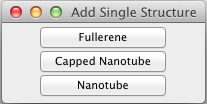
\includegraphics[scale= 0.6]{../../../../screens/nanocap_single_struct_win.png}
%\caption{\nanocap~structure list for adding a single structure}
%\label{c_single_structure_list}
%\end{figure}
%
%The capped nanotube structure added is a blank \textit{template} structure containing no points or atoms.  

The options to define the input parameters for the construction of the capped nanotube are displayed in the \textbf{Calculations--$>$Input} as shown in Fig~\ref{capped_nanotube_input_options}:

 \begin{figure}[h!]
\centering
\includegraphics[scale= 0.5]{../../../../screens/nanocap_capped_nanotube_input_win.png}
\caption{\nanocap~input options for a capped nanotube}
\label{capped_nanotube_input_options}
\end{figure}

The following input options can be set for the capped nanotube construction.
\begin{itemize}
 \item the chirality ($n,m$)
 \item the length of the nanotube (\AA)
 \item the number of cap carbon atoms and dual lattice points (or enabled the estimation based upon the nanotube density)
 \item the seed for the initial random cap point placement
 \item the force cutoff relating to the dual lattice force field (Section \ref{dforcefields})
 \end{itemize}
 
 
 
